\documentclass[review, doubleblind, 3p,
authoryear]{elsarticle} %review=doublespace preprint=single 5p=2 column
%%% Begin My package additions %%%%%%%%%%%%%%%%%%%

\usepackage[hyphens]{url}

  \journal{Computers, Environment and Urban Studies} % Sets Journal name

\usepackage{graphicx}
%%%%%%%%%%%%%%%% end my additions to header

\usepackage[T1]{fontenc}
\usepackage{lmodern}
\usepackage{amssymb,amsmath}
% TODO: Currently lineno needs to be loaded after amsmath because of conflict
% https://github.com/latex-lineno/lineno/issues/5
\usepackage{lineno} % add
  \linenumbers % turns line numbering on
\usepackage{ifxetex,ifluatex}
\usepackage{fixltx2e} % provides \textsubscript
% use upquote if available, for straight quotes in verbatim environments
\IfFileExists{upquote.sty}{\usepackage{upquote}}{}
\ifnum 0\ifxetex 1\fi\ifluatex 1\fi=0 % if pdftex
  \usepackage[utf8]{inputenc}
\else % if luatex or xelatex
  \usepackage{fontspec}
  \ifxetex
    \usepackage{xltxtra,xunicode}
  \fi
  \defaultfontfeatures{Mapping=tex-text,Scale=MatchLowercase}
  \newcommand{\euro}{€}
\fi
% use microtype if available
\IfFileExists{microtype.sty}{\usepackage{microtype}}{}
\usepackage[]{natbib}
\bibliographystyle{elsarticle-harv}

\ifxetex
  \usepackage[setpagesize=false, % page size defined by xetex
              unicode=false, % unicode breaks when used with xetex
              xetex]{hyperref}
\else
  \usepackage[unicode=true]{hyperref}
\fi
\hypersetup{breaklinks=true,
            bookmarks=true,
            pdfauthor={},
            pdftitle={Reproducible methods for modeling combined public transport and cycling trips and associated benefits: evidence from the biclaR tool},
            colorlinks=true,
            urlcolor=blue,
            linkcolor=blue,
            pdfborder={0 0 0}}

\setcounter{secnumdepth}{5}
% Pandoc toggle for numbering sections (defaults to be off)


% tightlist command for lists without linebreak
\providecommand{\tightlist}{%
  \setlength{\itemsep}{0pt}\setlength{\parskip}{0pt}}




\usepackage{subfig}
\usepackage{booktabs}
\usepackage{longtable}
\usepackage{array}
\usepackage{multirow}
\usepackage{wrapfig}
\usepackage{float}
\usepackage{colortbl}
\usepackage{pdflscape}
\usepackage{tabu}
\usepackage{threeparttable}
\usepackage{threeparttablex}
\usepackage[normalem]{ulem}
\usepackage{makecell}
\usepackage{xcolor}

\biboptions{authoryear}
\usepackage{url}
\usepackage{float}
\usepackage{booktabs}
\usepackage{longtable}
\usepackage{makecell}
\usepackage{multirow}

\begin{document}


\begin{frontmatter}

  \title{Reproducible methods for modeling combined public transport and
cycling trips and associated benefits: evidence from the biclaR tool}
    \author[CERIS]{Rosa Félix\corref{cor1}%
  \corref{cor1}%
  }
   \ead{rosamfelix@tecnico.ulisboa.pt} 
    \author[CERIS]{Filipe Moura%
  %
  }
   \ead{fmoura@tecnico.ulisboa.pt} 
    \author[ITS]{Robin Lovelace%
  %
  }
   \ead{r.lovelace@uleeds.uk} 
      \affiliation[CERIS]{CERIS, Instituto Superior Técnico -
Universidade de Lisboa. Av Rovisco Pais 1, 1049-001 Lisboa, Portugal}
    \affiliation[ITS]{Institute for Transport Studies, University of
Leeds. 34-40 University Rd, Leeds LS2 9JT, UK}
    \cortext[cor1]{Corresponding author}
  
  \begin{abstract}
  A high proportion of car trips can be replaced by a combination of
  public transit and cycling for the first-and-last mile. This paper
  estimates the potential for cycling combined with public transit as a
  substitute for car trips in the Lisbon metropolitan area and assesses
  its socio-environmental impacts using open data and open source tools.
  A decision support tool that facilitates the design and development of
  a metropolitan cycling network was developed (\emph{biclaR}). The
  social and environmental impacts were assessed using Health World
  Organization tools. The impacts of shifting car trips to public
  transport were also estimated and monetized. The results show that
  10\% of all trips could be made by cycling in combination with public
  transport. Shifting to cycling for the shorter first and last mile
  stages can reduce annual CO\textsubscript{2}eq emissions from 3,000 to
  7,500 tons/day, while for the public transport leg, the transfer from
  car avoids of up to 20,500 tons of CO\textsubscript{2}eq emissions per
  year. The estimated socio-environmental benefits are of €125 million
  to €325 million over 10 years. This evidence can support policymakers
  to prioritize interventions that reduce the reliance on private motor
  vehicles.\\
  \end{abstract}
    \begin{keyword}
    Active transport \sep Intermodality \sep First and last
mile \sep Health economic assessment \sep Environmental impacts \sep 
    Open data and methods
  \end{keyword}
  
 \end{frontmatter}

\hypersetup{citecolor=black}

\section{Introduction}\label{introduction}

Combining public transportation (PT) and cycling for the first and last
mile in metropolitan areas can replace a high proportion of private car
trips \citep{MARTENS2007326, van2021insights}. In The Netherlands, which
has the highest mode share of cycling in the world, cycling accounts for
more than a third of all trips to and from rail stations at the `home'
end of the journey, greatly increasing the ability of the transport
system \citep{RIETVELD200071}. This approach to reducing car dependency
and associated externalities requires interventions and programs to make
bicycling more appealing \citep{lapaix_role_2021}. The resulting public
investments can have significant social and environmental benefits
\citep{internationaltransportforum_integrating_2017}. Despite the
benefits of cycling-PT intermodality, the potential of this combination
is often overlooked in transport planning \citep{lapaix_role_2021}.

The potential of cycling as a complementary mode of PT is substantial
worldwide, especially in cities with established public transport
networks or substantial ambitions to develop them. In the Lisbon
metropolitan area (LMA) the largest metropolitan area in Portugal, the
modal share of cycling is low, but the potential for cycling as a
complementary mode of PT is high.

The Portuguese Government has established a national cycling strategy,
which outlines targets for the percentage of trips to be made by bicycle
in urban areas. Specifically, these targets aim for 4\% of all trips in
2025 and 10\% by 2030 \citep{ENMAC}. Moreover, the strategy emphasizes
that this increase should be achieved by substituting car trips for
bicycle trips, as a way to reduce the environmental and social impacts
of car use.

To support the implementation of this strategy, the Lisbon's
Metropolitan Department of Transport commissioned
\emph{biclaR}\footnote{See
  \href{https://biclar.tmlmobilidade.pt/}{biclar.tmlmobilidade.pt}.}, a
decision support tool that facilitates the planning, design, and
development of a metropolitan cycling network \citep{felix2023}.

\emph{biclaR} builds on the Propensity to Cycle Tool\footnote{See
  \href{https://www.pct.bike/}{pct.bike}.} (PCT), a web application and
research project funded by the UK's Department for Transport in 2015
which launched nationally in 2017 as part of the government's Cycling
and Walking Investment Strategy. The PCT initially used only
origin-destination data for commuting trips as the basis of estimates of
cycling potential at zone, route and route network levels
\citep{lovelace2017}. The PCT has been extended to include cycling
potential for travel to school in England \citep{goodman2019} and other
trip types in other countries.\footnote{See
  \href{https://www.npt.scot}{npt.scot} and
  \href{https://cruse.bike}{cruse.bike} for examples of the PCT in
  Scotland and Ireland that include estimates of cycling for other
  purposes.} However, to the best of our knowledge, this is the first
time that the method has been integrated with public transport data
using multi-modal routing to estimate the potential and benefits of
multi-stage cycling and PT trips.

This paper estimates the potential for combining cycling and PT to
substitute car trips in the LMA. After presenting the methods used, we
assess its socio-environmental impacts using open data and open-source
tools.

\section{Methods}\label{methods}

\subsection{Case Study}\label{case-study}

According to the latest mobility survey conducted in 2018 \citep{IMOB},
the LMA registered a total of 5.3 million daily trips, with only 0.5\%
by bicycle. Car modal share was 58.4\%, while PT accounted for 15.5\%
(see Figure \ref{fig:mododist}). The number of intra-municipal trips ---
with origin and destination in the same municipality --- amounts to 3.5
million trips. This exceeds the number of inter-municipal trips (1.8
million trips), involving travel between different municipalities. Cars
and public transport are the most used modes for intercity trips, with
cars being the predominant choice for all journeys. 53\% trips are up to
5 km distance, and 71\% up to 10 km. Nevertheless, 29\% of trips are
longer than 10 km, which requires the use of motorized modes, or active
modes in combination with public transport.

Regarding cycling trips in the LMA, 55\% are up to 5 km, and 88\% are up
to 10 km. These values are not in line with the typically found in
cycling distance decay curves, which show a high percentage of trips are
up to 5 km (\textasciitilde75\%), and a smaller proportion up to 10 km
\citep{krizek2007detailed, larsen2010beyond, DDfunction2023}. This may
be due to the low cycling modal share in the LMA - even more limited in
the sample survey, which may be biased towards shorter trips.

\begin{figure}
\subfloat[In percentage\label{fig:mododist-1}]{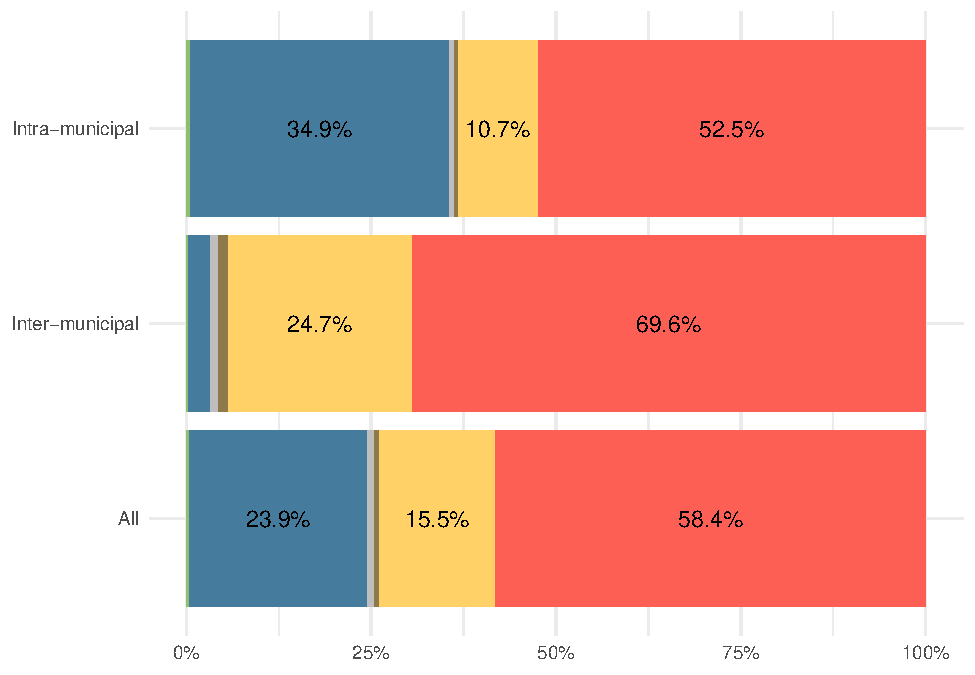
\includegraphics[width=0.5\linewidth,]{PaperCEUS_rev1_files/figure-latex/mododist-1} }\subfloat[In total\label{fig:mododist-2}]{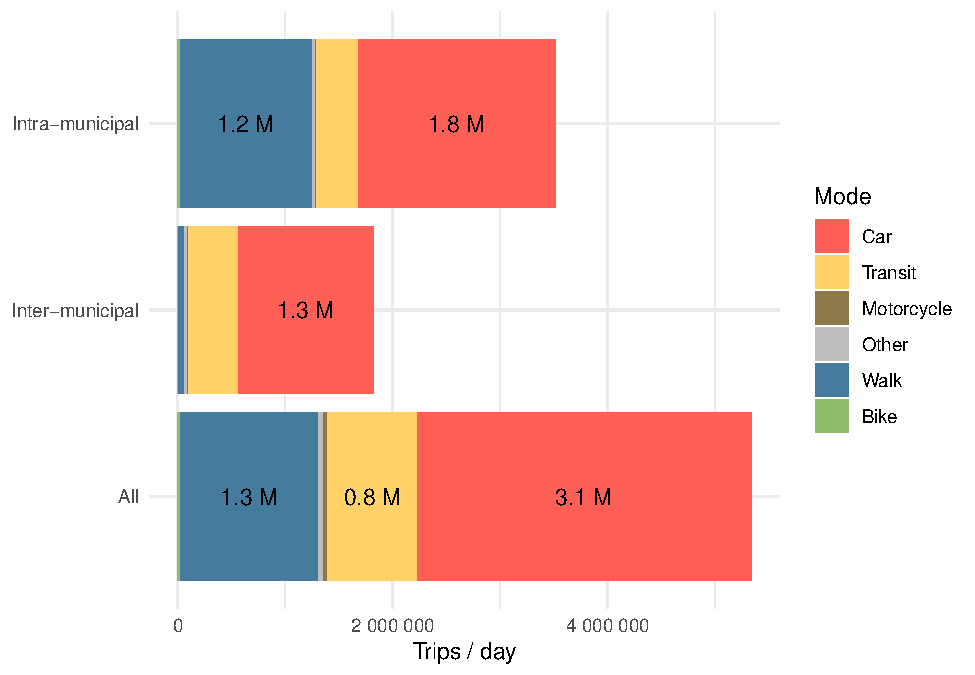
\includegraphics[width=0.5\linewidth,]{PaperCEUS_rev1_files/figure-latex/mododist-2} }\caption{\label{mododist}Trips in the LMA by inter/intra municipal and mode, according to the travel survey.}\label{fig:mododist}
\end{figure}

\textbf{TO-DO}

\begin{itemize}
\tightlist
\item
  mais mapas:
\item
  Densidade populational - nº de viagens
\item
  Pares OD - desire lines width
\end{itemize}

\subsection{Modeling Origin-Destination
trips}\label{modeling-origin-destination-trips}

The mobility survey data \citep{IMOB} is the basis of the baseline
scenario and trip rates presented in this paper. Conducted in the
pre-pandemic period (2017), this OD dataset represents the most
comprehensive and up-to-date information on urban mobility in Portuguese
metropolitan areas (Lisbon and Porto).

We used `jittering' to disaggregate the OD data, resulting in a wide
spatial distribution of trip origins and destinations
\citep{Lovelace2022Jittering}. The method works by sampling `sub-points'
(nodes on the transport network represented in OpenStreetMap in this
case) and using these instead of a single point (typically the centroid)
to represent trip origins and destinations for each zone. This method
then distributes the trips to desire lines connecting the subpoints
based on a `disaggregation threshold' which determines the maximum
number of trips that can be represented by a single desire line.

Using the
\href{https://github.com/dabreegster/odjitter}{\texttt{odjitter} R
package}, we disaggregated the OD data into desire lines reprenting a
maximum of 100 trips each. Figure \ref{fig:jitter} illustrates the
contrast between trip representation through the traditional method,
which connects a single desire line between each district, and the
presentation achieved through the randomization and disaggregation of
trips between districts, specifically for the Lisbon metropolitan area.

\begin{figure}

{\centering 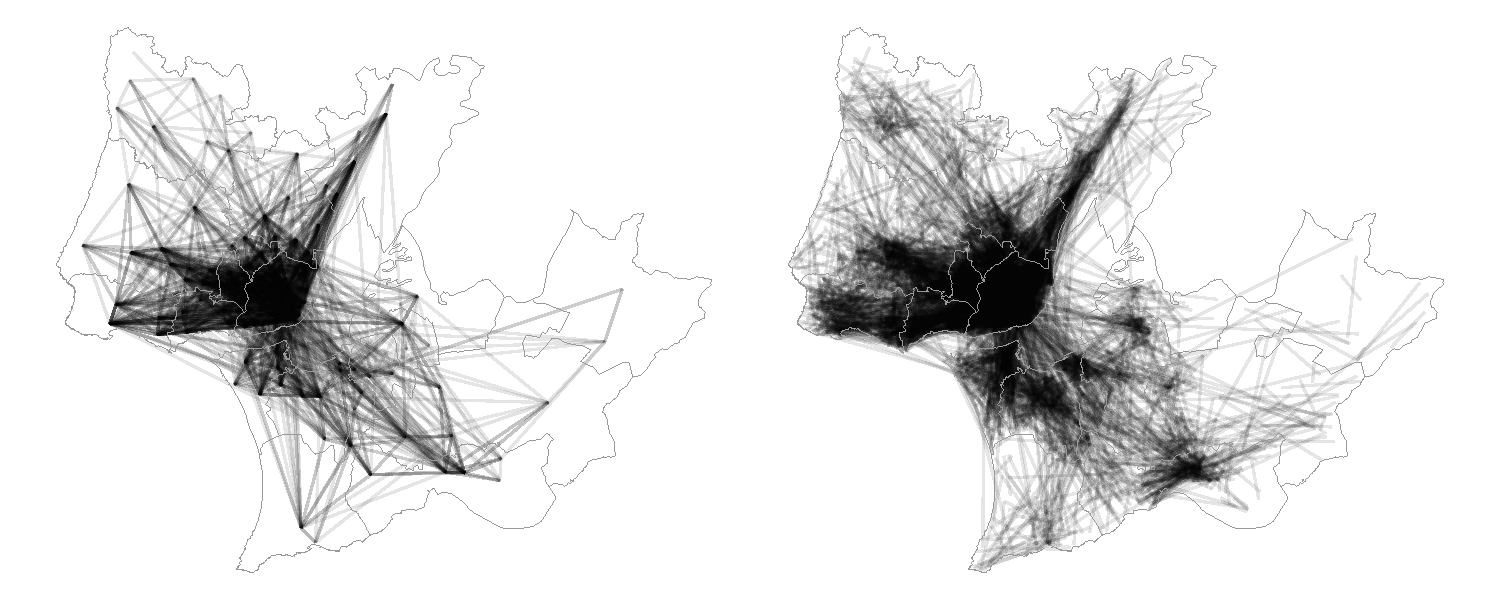
\includegraphics[width=1\linewidth,]{img/jitter_cairo} 

}

\caption{Flow-weighted random sample of 10,000 desire lines in the Lisbon metropolitan area between districts of the 18 municipalities, without jittering (left) and with jittering (right).}\label{fig:jitter}
\end{figure}

The jittering pre-processing stage generates a more realistic
representation of the trips undertaken than the traditional
centroid-based approach but does not precisely capture the exact spatial
distribution of trips. Even where such datasets exist, they cannot be
shared for research due to data privacy regulations.

\subsection{Modeling routes}\label{modeling-routes}

The mobility survey collects the origin and destination of trips but
does not include the respective routes. Modeling the realistic
cycling-PT routes between OD pairs depends on assumptions regarding the
characteristics of the cycling and road networks and the location of
public transport interfaces. Other constraints regarding the behavior of
potential cyclists determine the routing results. For example, such
restrictions can favor low speed, low traffic streets, more direct
routes, and less steep paths, among others, which are suitable for
cycling.

The selected route choice algorithm was the
\href{https://ipeagit.github.io/r5r/}{\texttt{r5r} R package}
\citep{r5r}, which allows for great flexibility in configuring estimated
route types, and which proven to provide most accurate route networks
for the city of Lisbon \citep{Lovelace2022exploring}. \texttt{r5r} can
calculate multi-modal routes using PT combined with other modes. It
enables the identification of the most direct or safest cycling routes,
using the Level of Traffic Stress\footnote{see
  \href{https://docs.conveyal.com/learn-more/traffic-stress}{docs.conveyal.com/learn-more/traffic-stress}.}
(LTS) scale, ranging from 1 to 4, where 1 corresponds to the quietest
(e.g., off-road cycle paths) and 4 corresponds to the least quiet (e.g.,
routes shared with motorized traffic). The routes were estimated for the
base scenario for both types of networks: \emph{direct} and \emph{safe},
using LTS 4 and LTS 3, respectively. Different routing profiles enable
decision-makers to plan for different bicycle user typologies and/or for
different city cycling maturity levels \citep{felix2017}.

The \texttt{r5r} model used the OpenStreetMap road network and the GTFS
metropolitan data aggregated and validated. This information is crucial
for an accurate PT trip and route estimation. A digital elevation model,
from the European Space Agency's COPERNICUS mission, was used to include
street gradient information, as a weight in cycling routing. The cycling
potential trips for the two national strategic targets (4\% and 10\%)
were estimated from the 2017 cycling and car trips (both as a driver and
as a passenger), the baseline scenario.

The routes were then overlaid and aggregated by segments, using
\href{https://docs.ropensci.org/stplanr/reference/overline.html}{\texttt{stplanr\ overline()}
R function}.

\subsection{Modeling intermodality}\label{modeling-intermodality}

The intermodality scenario considers trips made by PT in which cycling
is used for the first and last legs. We restricted our analysis to the
first and last legs with a combined length of up to 5 km (for example: 1
km from origin to interface \emph{A} plus 4 km from interface \emph{B}
to destination). Furthermore, we have imposed restrictions on PT usage,
limiting it to trips without PT transfers, and within a duration of up
to 2 hours (120 minutes). Additionally, we have only included PT modes
that can easily accommodate bicycles, such as trains, ferries, trams,
and inter-municipal bus lines equipped with bike racks (Figure
\ref{fig:map1}).

This conservative approach was adopted to capture the fact that cycling
stages as part of a multi-modal trip are likely to be shorter than
cycling-only trips \citep{vanmil_insights_2021}. Additionally,
\citet{Leferink2017} found that the bicycle is most attractive option as
a first and last mile mode when the distance ranges from 3 to 5 km, as
observed across various comparative studies. This restrictions are based
on the assumption that 5 km is a plausible maximum distance that people
are willing to travel by bike as part of a longer journey. This applies
especially for cycling beginners shifting from cars, who are less likely
to be confident and experienced cyclists than the existing cyclists.

These restrictions can be eased in the future when testing more
developed policy interventions to enhance intermodality between cycling
and PT, considering both the vehicle and infrastructure perspectives.

\begin{figure}

{\centering 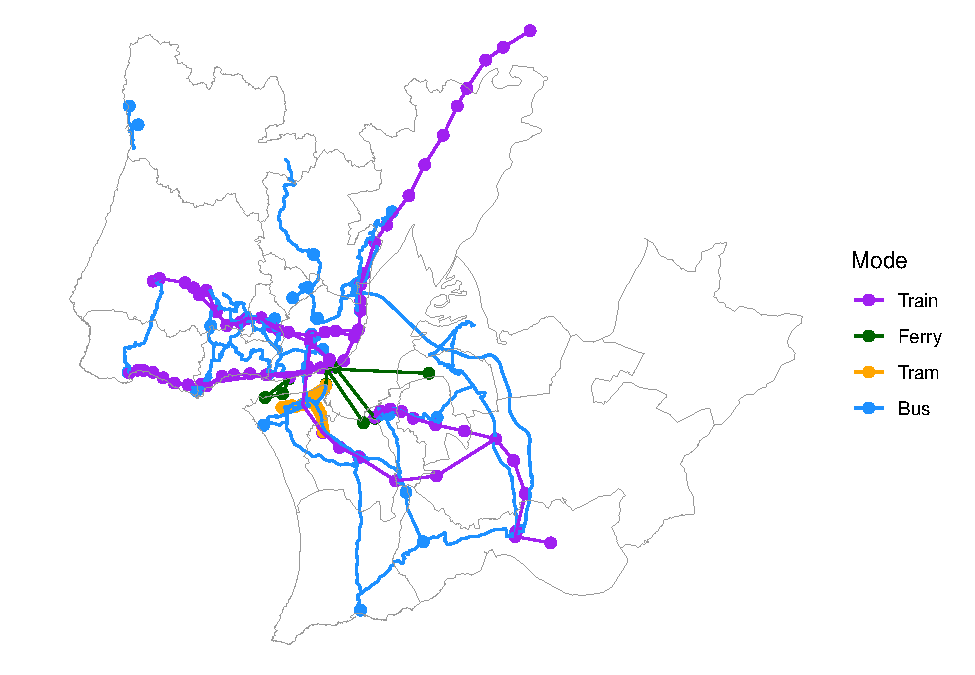
\includegraphics[width=0.6\linewidth,]{PaperCEUS_rev1_files/figure-latex/map1-1} 

}

\caption{Interfaces and lines considered, by transport mode, in the Lisbon metropolitan area.}\label{fig:map1}
\end{figure}

Figure \ref{fig:map2} illustrates the resulting bicycle routes to access
the main PT interfaces in the LMA. It is noticeable the high potential
of the train interfaces to attract car-to-PT substituting trips.

\begin{figure}

{\centering 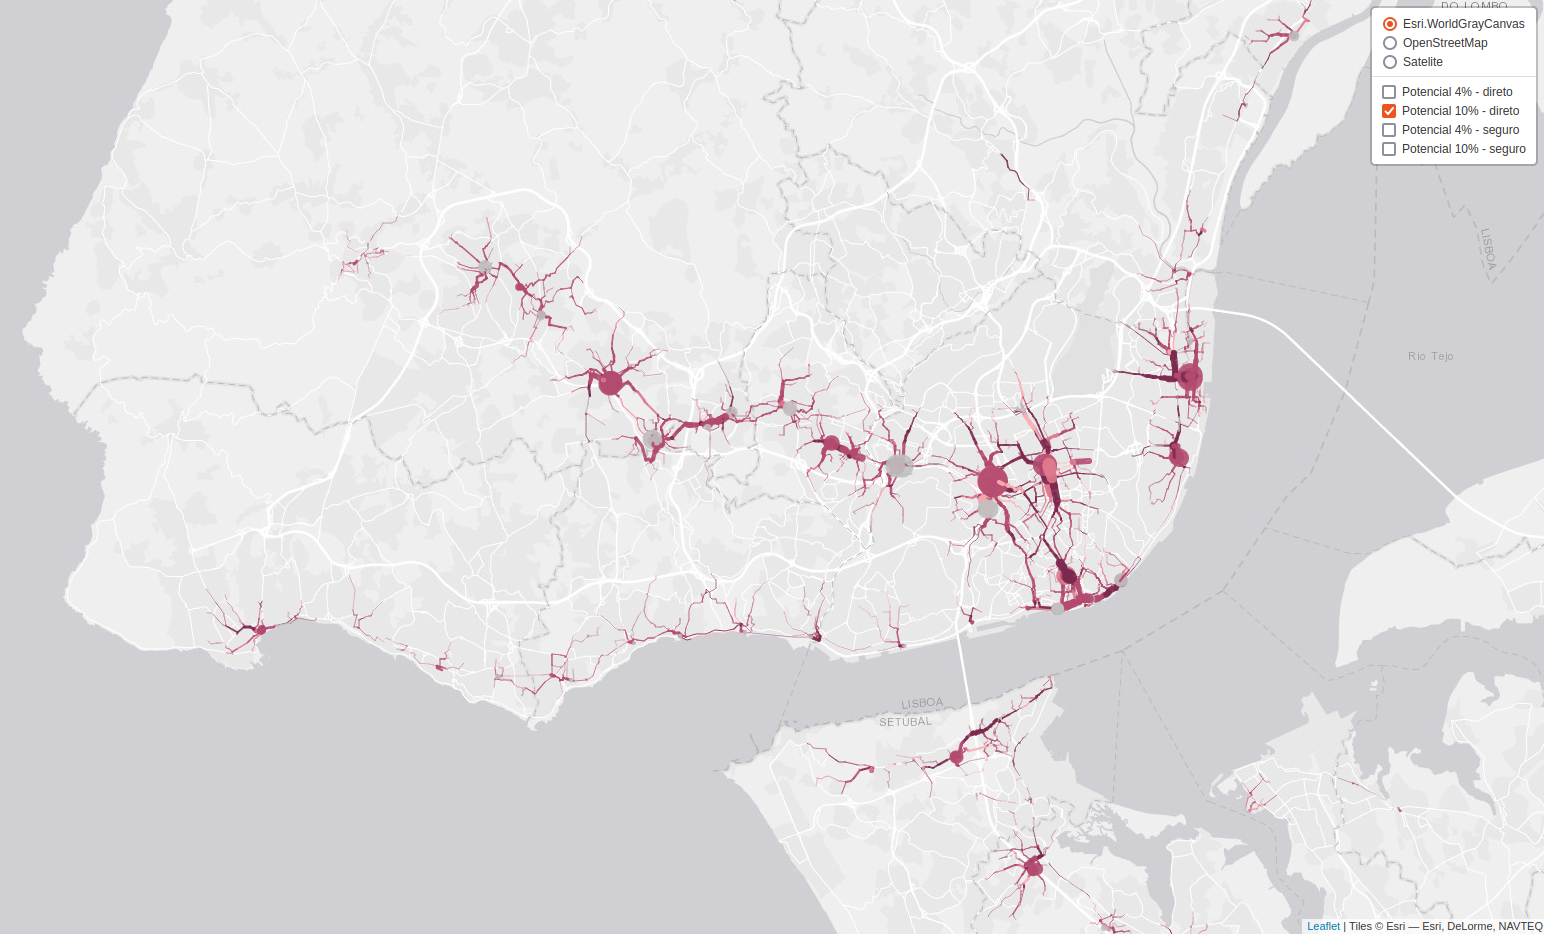
\includegraphics[width=0.8\linewidth,]{img/map2} 

}

\caption{Bike routes with the highest potential to serve as first and last leg when replacing cycling and PT from car trips (screenshot of the interactive online tool). Larger the line width, higher the segment's car to bicycle shift potential. Darker the line color, lower the quietness level.}\label{fig:map2}
\end{figure}

\subsection{Modelling car shift to bicycle-PT - here or
before??}\label{modelling-car-shift-to-bicycle-pt---here-or-before}

It is essential to note that our approach is not predictive but
scenario-based, providing a range of potential outcomes regarding the
target (\% of cycling tips) and the routing profile (safe or direct
routes), rather than a single forecast. These scenarios are rooted in
the explicit national cycling targets, assuming that the potential for
cycling is proportional to the reduction of car trips. Thus said, we do
not predict the generation of new trips, but the substitution of car
trips by cycling in combination with PT, considering the potential of
the first and last mile of these journeys to be made by bicycle.
Additionally, we do not model changes in the baseline PT trips, under
the implicit assumption that the initial and final stages of these trips
remain unaltered.

A strength of this \emph{backcasting} approach is that we can simulate
the aggregate travel patterns that would meet particular policy
objectives, and explore what the implications could be for the public
transport system and provision of safe cycling infrastructure to public
transport nodes at regional, local authority and, importantly from a
local transport planning practitioner perspective, corridor level.

\subsection{Assessing socio-environmental
benefits}\label{assessing-socio-environmental-benefits}

Following the clearly established national strategy, we estimated the
socio-environmental potential impacts of shifting car trips by bicycle
in combination with PT, in the LMA, for the two targets (4\% and 10\%).

For the \emph{cycling legs of the journey} (first and last legs),
socio-environmental impacts were estimated, using the Health Economic
Assessment Tool (HEAT) for Cycling v5.2 \citep{HEAT}, from the World
Health Organization, and the
\href{https://github.com/HEAT-WHO/HEAT_heatr_api}{\texttt{HEATaaS} R
package}\footnote{\texttt{HEATaaS} is under development. For more
  information contact
  \href{https://heatwalkingcycling.org}{heatwalkingcycling.org}.}. The
use of this package made it possible to run multiple scenarios with few
changes in input values, making the interaction with HEAT more reliable
when reproducing runs.\\
The HEAT tool provided estimates on the shifting from car to cycling for
a short term time horizon (i.e., one year) and the long term (i.e., ten
years). It estimates the differences between two considered scenarios.
In this case: one baseline scenario, with data from the mobility survey,
and one cycling potential scenario in which targets of 4\% and 10\% of
cycling levels were achieved, transferred from car trips. We considered
two dimensions: \emph{social} --- including the physical activity, air
pollution exposure, and road casualties; and \emph{environmental} ---
including CO\textsubscript{2}eq emissions and other pollutants.

For the \emph{second leg of the journey}, we estimate the environmental
impacts of shifting car trips to PT (between the PT interfaces).

To estimate the car emissions, we used the EMEP/EEA's COPERT software v5
methods and reference values \citep{COPERT} for a Tier 3 detail level.
We used a family-size vehicle, EURO standard, and gasoline or diesel
fuel. All trips were considered to be made under urban conditions and at
an average speed of 15 km/h during rush hour periods. Since the average
distance traveled per trip influences the overconsumption and emissions
from cold-start engine operation, we estimated energy and emission
factors for different ranges of trips at 500-meter intervals.\\
An equation was then used to calculate emission factors for the two
types of fuel, for each type of pollutant, whose explanatory variables
are driving speed (\(speed\), in km/h) and average trip distance
(\(l_{trip}\), in km/trip). Thus, the emission factors
(\(EF_{fuel,l_{trip},speed}\), in g/km) can be calculated using equation
\ref{eq:fatoremissaoauto}.

\begin{equation}\label{eq:fatoremissaoauto}
{EF}_{fuel,l_{trip},speed} = a + b\cdot {speed} + c\cdot l_{trip}
\end{equation}

Emission factors are estimated for the following air pollutants: CO,
NO\textsubscript{X}, VOC, and PM\textsubscript{10}. Emission factors of
the main greenhouse gases (GHG) are also estimated: CO\textsubscript{2},
CH\textsubscript{4} and N\textsubscript{2}O, converted in
CO\textsubscript{2}eq by the following relationship\footnote{The weights
  correspond to the Global Warming Potentials (GWP) defined for a
  100-year period by the IPCC in its
  \href{https://www.ipcc.ch/report/ar5/}{5th Assessment Report}.}:
\(EF_{CO_2eq} = EF_{CO_2} + 28\cdot EF_{CH_4} + 265\cdot EF_{N_2O}\).
The CH\textsubscript{4} and N\textsubscript{2}O emission factors do not
vary with travel speed. The PM\textsubscript{10} emission factor does
not vary with trip distance.

The used values consider that 64\% of the car fleet was diesel in
2022\footnote{See
  \href{https://smi.ine.pt/Indicador/Detalhes/10837?LANG=EN}{Statistics
  Portugal: Stock road vehicles statistic}.}. In addition, we assumed an
occupancy rate of 1.6 passengers \emph{per} car \citep{IMOB}. Finally,
the final emissions for each trip (\(E_{pollutant}\), in g/trip) are
derived from the equation \ref{eq:emissaoauto}.

\begin{equation}\label{eq:emissaoauto}
{E}_{pollutant} = {EF}_{fuel,l_{trip},speed}\cdot l_{trip}
\end{equation}

Regarding PT, we considered the emission factor values reported in the
environmental and sustainability reports of the PT operators in the LMA
\citep{Carris2019s, Metro2019s, CP2019s, Transtejo2014}. In particular,
for the urban train and tram -- with 100\% electric traction -- only
CO\textsubscript{2}eq emissions were considered (resulting from the
production of electricity, considering a ``well-to-tank'' approach),
since the other pollutants are not emitted locally.

The conversion of avoided emissions into avoided welfare loss and
respective monetary valuation was based on the EU Guide to Cost-benefit
Analysis \citep{EuropeanCommission2014} and the best up-to-date
reference values for the various gases
\citep{EuropeanCommission2014, bickel2006, UNITE}: 8.44 €/ton for CO,
2,867.85 €/ton for NO\textsubscript{X}, 340,969.27 €/ton for
PM\textsubscript{10}, 7,169.62 €/ton for VOC and 35.85 €/ton for
CO\textsubscript{2}eq. The social impacts are in avoided premature
mortality. This result is finally monetized using the \emph{Statistical
Value of Life} for Portugal: €3,055,358/fatality \citep{ANSR2021}. We
updated all the monetary reference values of the literature based on the
annual inflation rate in Portugal for 2022\footnote{See
  \href{https://www.ine.pt/xportal/xmain?xpid=INE&xpgid=ipc}{Statistics
  Portugal tool for inflation rate estimates between years}.}, and our
10-years estimations assumed a discount rate of 5\% and inflation of
3\%. See \hyperref[research-data]{Research Data} for all the input
values we used.

\section{Results and Discussion}\label{results-and-discussion}

Table \ref{tab:summary1} presents the LMA total daily trips that can be
made with cycling + TP combination (with the aforementioned
restrictions), the trips in the baseline scenario and corresponding new
daily trips to achieve the national strategy targets (4\% and 10\%), for
different route profiles. For the cycling legs of the journey (first and
last legs), the environmental avoided emissions and monetized
socio-environment (SE) benefits are presented in Table
\ref{tab:summary1b}, resulting from replacing car trips with cycling.

\begin{table}

\caption{\label{tab:summary1}\label{summary1}Summary of the cycling potencial of the intermodality scenario. Values in 'trips/day'.}
\centering
\begin{tabular}[t]{llr>{\raggedleft\arraybackslash}p{7em}>{\raggedleft\arraybackslash}p{7em}}
\toprule
Target & Routing & Total trips & Baseline Cycling + PT & Potencial Cycling + PT\\
\midrule
4\% & safe & 538 514 & 2 312 & 20 385\\
4\% & direct & 500 880 & 2 274 & 18 944\\
10\% & safe & 538 514 & 2 312 & 52 323\\
10\% & direct & 500 880 & 2 274 & 48 609\\
\bottomrule
\end{tabular}
\end{table}

\begin{table}

\caption{\label{tab:summary1b}\label{summary1b}Summary of the cycling potencial of intermodality scenario and its socio-environmental benefits for the cycling legs.}
\centering
\begin{tabular}[t]{ll>{\raggedleft\arraybackslash}p{6em}>{\raggedleft\arraybackslash}p{6em}>{\raggedleft\arraybackslash}p{6em}>{\raggedleft\arraybackslash}p{6em}}
\toprule
Target & Routing & Avoided Mortality (deaths/yr) & Social benefits (k€/yr) & Avoided CO2eq (ton/yr) & Environmental benefits (k€/yr)\\
\midrule
4\% & safe & 4.1 & 12 717 & 2 958 & 238\\
4\% & direct & 4.0 & 12 441 & 3 004 & 241\\
10\% & safe & 10.0 & 32 820 & 7 590 & 610\\
10\% & direct & 10.0 & 31 800 & 7 694 & 618\\
\bottomrule
\end{tabular}
\end{table}

For both \emph{direct} and \emph{safe} route profiles, 10\% of the daily
trips have the potential to be made by a combination of PT and cycling,
even given the travel restrictions considered (up to 5 km on bike, up to
2 hours, no possible transfers between PT). This unveils the potential
of cycling as a complementary mode of PT, with the potential to uptake
the number of PT trips within the LMA area by as much as 6.3\% (in
addition to the 825 thousand PT trips reported in the mobility survey).

Table \ref{tab:summary21} shows the potential trips by PT mode to
replace the second leg of the journey, in combination with cycling.
Train offers the greatest potential for substitution (88\%). When
comparing the existing PT interfaces (Figure \ref{fig:map1}) with the
bike routes with highest potential to serve as first and last legs
(Figure \ref{fig:map2}) it becomes clear that the Train interfaces are
the ones that have the highest potential to attract car-to-PT
substituting trips, if their accessibility by bicycle is improved to
become safer.

\begin{table}

\caption{\label{tab:summary21}\label{summary21}Summary of the potential of replacing car trips with cycling in combination with PT, disagregated by PT mode. Values in 'trips/day'.}
\centering
\begin{tabular}[t]{>{\raggedright\arraybackslash}p{4.5em}>{\raggedright\arraybackslash}p{4.5em}>{\raggedleft\arraybackslash}p{4.5em}>{\raggedleft\arraybackslash}p{4.5em}>{\raggedleft\arraybackslash}p{4.5em}>{\raggedleft\arraybackslash}p{4.5em}>{\raggedleft\arraybackslash}p{4.5em}}
\toprule
Target & Routing & Potential & Bus & Ferry & Train & Tram\\
\midrule
4\% & safe & 20 385 & 573 & 285 & 17 716 & 1 811\\
4\% & direct & 18 944 & 593 & 313 & 17 093 & 946\\
10\% & safe & 52 323 & 1 452 & 712 & 45 588 & 4 571\\
10\% & direct & 48 609 & 1 520 & 781 & 43 932 & 2 375\\
\bottomrule
\end{tabular}
\end{table}

The benefits are spatially unevenly distributed across the LMA, as shown
in Figure \ref{fig:mapzones}.

Table \ref{tab:summary22} presents emissions reductions and associated
economic benefits associated with the second (PT) leg of trips. The
shift from private car associated with thes PT segments would reduce
CO\textsubscript{2} equivalent emissions by 8,500 to 20,800 tons
annually, valued in €1.4 million to €3.5 million yearly, for the 4\% and
10\% targets, respectively.

\begin{table}

\caption{\label{tab:summary22}\label{summary22}Summary of the avoided emmissions (ton/year) and corresponding monetization (thousand €) by replacing car trips with PT, in the second leg.}
\centering
\begin{tabular}[t]{ll>{\raggedleft\arraybackslash}p{3.5em}>{\raggedleft\arraybackslash}p{3.5em}>{\raggedleft\arraybackslash}p{3.5em}>{\raggedleft\arraybackslash}p{3.5em}>{\raggedleft\arraybackslash}p{3.5em}r}
\toprule
Target & Routing & CO2eq & CO & PM10 & NOx & VOC & Value (k€)\\
\midrule
4\% & safe & 8 593 & 17 & 1.9 & 27 & 0.8 & 1 425\\
4\% & direct & 8 702 & 18 & 2.0 & 28 & 0.8 & 1 453\\
10\% & safe & 20 627 & 42 & 4.6 & 65 & 2.0 & 3 431\\
10\% & direct & 20 793 & 42 & 4.7 & 66 & 1.9 & 3 487\\
\bottomrule
\end{tabular}
\end{table}

The sum of CO\textsubscript{2}eq avoided emissions from the potential
car trips shifted to bike (first-and-last legs) in combination with PT
(second leg) in the LMA is presented in Table \ref{tab:summaryall}, for
both national cycling strategy targets and routing profiles, and the
socio-environmental benefits monetized in €, for a 1-year and 10-year
time periods.

\begin{table}

\caption{\label{tab:summaryall}\label{summaryall}Summary of the avoided CO2eq emmissions (ton/year) and the estimated social and environmental benefits (monetized in thousand €) by replacing car trips with cycling in combination with PT.}
\centering
\begin{tabular}[t]{ll>{\raggedleft\arraybackslash}p{8em}>{\raggedleft\arraybackslash}p{8em}>{\raggedleft\arraybackslash}p{8em}}
\toprule
Target & Routing & Avoided CO2eq (tons) & SE Benefits 1yr (k€) & SE Benefits 10yrs (k€)\\
\midrule
4\% & safe & 11 551 & 14 380 & 127 534\\
4\% & direct & 11 706 & 14 135 & 125 016\\
10\% & safe & 28 217 & 36 861 & 325 814\\
10\% & direct & 28 487 & 35 905 & 318 062\\
\bottomrule
\end{tabular}
\end{table}

Shifting from car to cycling in combination with PT can reduce annual
CO\textsubscript{2}eq emissions by 11,500 to 28,500 tons per year. These
figures represent a 2.7\% reduction in Lisbon's transport emissions
\citep{LisboaENova}, a small but important component of wider transport
decarbonization measures. The 10-year socio-environmental benefits
account for €125 million to €325 million, depending on the cycling
targets.

The environmental impacts represent less than 2\% of the
socio-environmental benefits (in value) from replacing car trips to
bicycle in first-and-last legs. For the PT segment, we did not estimate
the social impacts from substituting car trips. One of the main
socio-environmetal benefits, valued after monetization, comes from the
increase in physical activity \citep{Felix2023ES}. Although there are
also social benefits form shifting car trips to PT, its health benefits
would not be as high as shifting to cycling. The literature shows that
the Metabolic Equivalent Tasks (MET) for ``riding in a bus or a train''
is 1.3 plus the ``walking for transportation'' as 3.5, while ``driving a
car'' is 2.5 \citep{MET2011}. The difference between these activities -
shifting from car to PT - is not very obvious when compared to shifting
from car to cycling, whose MET is about 6.8. Nevertheless, future works
should also encompass the estimation of the social impacts for the PT
leg of the journey, shifting from car.

The emissions of CO\textsubscript{2}eq that are avoided during both the
initial and final journey segments account for about 74\% of the
emissions avoided during the PT segment. This finding, while expected --
due the zero cycling emissions, should not be overlooked when promoting
the PT use. Improving the safe accessibility to PT interfaces to
cyclists and providing bicycle-friendly amenities such as parking
facilities can potentially lead to a higher reduction in
CO\textsubscript{2}eq emissions, compared to a scenario where
individuals shift from car travel to car + PT combination.

Our findings show that cycling \emph{in combination} with PT could
replace 10\% of current LMA trips, with an additional 6\% of PT journeys
prone to further substitution, based on conservative assumptions.
Although this paper does not address the designing specific solutions,
our findings indicate a potential surge in demand (+6.3\%) of public
transport interfaces to align with the national strategies. This added
demand is conceptually driven from individuals utilising bicycles,
either personal or shared, which would be parked at the PT stations.
Consequently, operators and public space managers would face the
challenge of accommodating this increased demand for bicycle parking
and/or docks from a bike sharing system, since this availability plays a
crucial role in the decision-making process of individuals to use
combined bike-train \citep{jonkeren2021bicycle}. Additionally, they may
need to explore options to enhance bicycle carriage capacity on public
transport services, ensuring alignment with national targets.

\section{Generalizability and
limitations}\label{generalizability-and-limitations}

This paper focus primarily on the potential for replacing trips
currently made by car with combined cycling and public transport trips,
and the associated social and environmental benefits, showcasing the
potential impact of facilitating the first-and-last mile to PT
interfaces. While the results are specific to the Lisbon Metropolitan
Area, the approach is designed to be generalizable to other metropolitan
areas.

An important aspect of the approach from a generalizability perspective
is that it has specific data requirements, including origin-destination,
road network, and the GTFS data. Such datasets are available to
transport planners in many areas. In areas where such datasets do not
exist, the value of research such as this could provide a motivation to
collect and open-up transport data. For this study we have used
Portugal's national cycling targets as the basis of the scenarios; the
approach can be adapted to other targets, or to other policy goals, such
as reducing congestion or improving air quality.

Nevertheless, the extent of the potential shift from car to PT is highly
dependent on the distances typically travelled in such contexts, and the
availability of PT services - which can vary significantly between
regions, and for which we are not assuming any change in this study. For
instance, we considered only the inter-municipal bus services that
accommodate bicycles on board. Future research could explore the
potential of equipping other regional bus services with this feature and
analyse their attractiveness, combined with cycling, to address current
car trip demands.

A strength of the approach is that there is no requirement for sensitive
individual trip level data to reproduce the approach in other cities.
However, we acknowledge that this approach has limitations. The approach
cannot show exactly which trips are being replaced, in terms of the age
of people making the trips, the types of car they drive, and other
individual or vehicle level variables. We assumed uniformity in the type
of vehicle for all replaced car journeys, albeit with variations in the
fuels utilised. Additionally, we assumed consistency in the health
impacts across all individuals for the replaced car trips. This approach
is a simplification of reality to enable the analysis of a large region
on available computing resources. Future work could seek to increase the
resolution of the results, and move towards a more individual-level
analysis, for example by using agent and activity-based models using
tools such as MATSim \citep{MATSim}. This option would require
substantial resources outside the scope of this study; another way to
improve the spatial resolution of results would be to use higher
resolution `subpoints' as the basis of the desire line `jittering'
process. We would also like to explore the potential for probabilistic
routing to improve the spatial resolution of the results.

A further refinement could be to differentiate between `simpler'
no-transfer PT trips (which require less person effort) and more arduous
multi-transfer PT trips, using the same methods, by relaxing the
assumption of no-transfers between PT modes in the routing engine. This
would lead to a larger number of total daily trips that can be made by
cycling + PT, in particular in locations where the PT network is less
complex and requires more transfers. We could also set a different
maximum length of cycling stage, extending the bicycle catchment area.
However, despite the added value of a sensitivity analyses, they would
also increase the overall complexity, and would have an impact on the
explainability of the results to be used by policy makers.

\section{Conclusion}\label{conclusion}

This paper estimated the potential for combining cycling and PT to
substitute car trips in the LMA, while achieving the national cycling
targets and supporting decarbonization goals. It has become
progressively more common to establish strategic plans, at national,
regional or municipal level, to mitigate climate change. Among these,
the Sustainable Urban Mobility Plans (SUMP\footnote{See
  \href{https://www.eltis.org/mobility-plans/sump-concept}{eltis.org/mobility-plans/sump-concept}}),
promoted by the European Commission, are becoming popular in Europe,
although authorities are designing documents of this sort all over the
world. The definition of targets associated with a timeframe for
reducing dependence on the individual motorized vehicle, or targets for
the use of active modes such as walking and cycling, are too often not
accompanied by estimates of their social, environmental and economic
impacts. It is important for authorities and practitioners to know how
to estimate those impacts, which tools are available to support them in
the process, and what results to expect.

This paper quantifies the benefits of replacing car trips with cycling,
in combination with public transport. The case study of the Lisbon
metropolitan area demonstrates that cycling-PT integration can help meet
the national targets set for bicycle use of 4\% and 10\% by 2025 and
2030, respectively.

The quantification of benefits can support policy-makers in prioritizing
interventions to reduce the reliance on private motorized modes of
transportation. The presentation of the results in an open access web
application will help to inform and explain decisions. Furthermore, the
provision of datasets resulting from this project provides a foundation
for further research and development of new tools and methods. The
methods are reproducible and based on open source software, which can be
applied to other cities and metropolitan areas, supporting the
decarbonization of transport systems internationally.

\section*{Acknowledgements}\label{acknowledgements}
\addcontentsline{toc}{section}{Acknowledgements}

{[}\emph{blind}{]}

\section*{Research data}\label{research-data}
\addcontentsline{toc}{section}{Research data}

The data and the code to reproduce the results will be made available
upon publication.

\renewcommand\refname{References}
\bibliography{bibliography.bib}


\end{document}
